\subsection{Structure}

\paragraph{}There are several types of commercial structures. According to the needs of the project, the structure that Astrea is looking for has to be very flexible regarding the placement of the subsystems. It has to adapt to the needs of the project continuously given that the satellite do not have a typical configuration.\\
A basic schematics can be found in the figure \ref{epsschematics}.

\begin{figure}[h!]
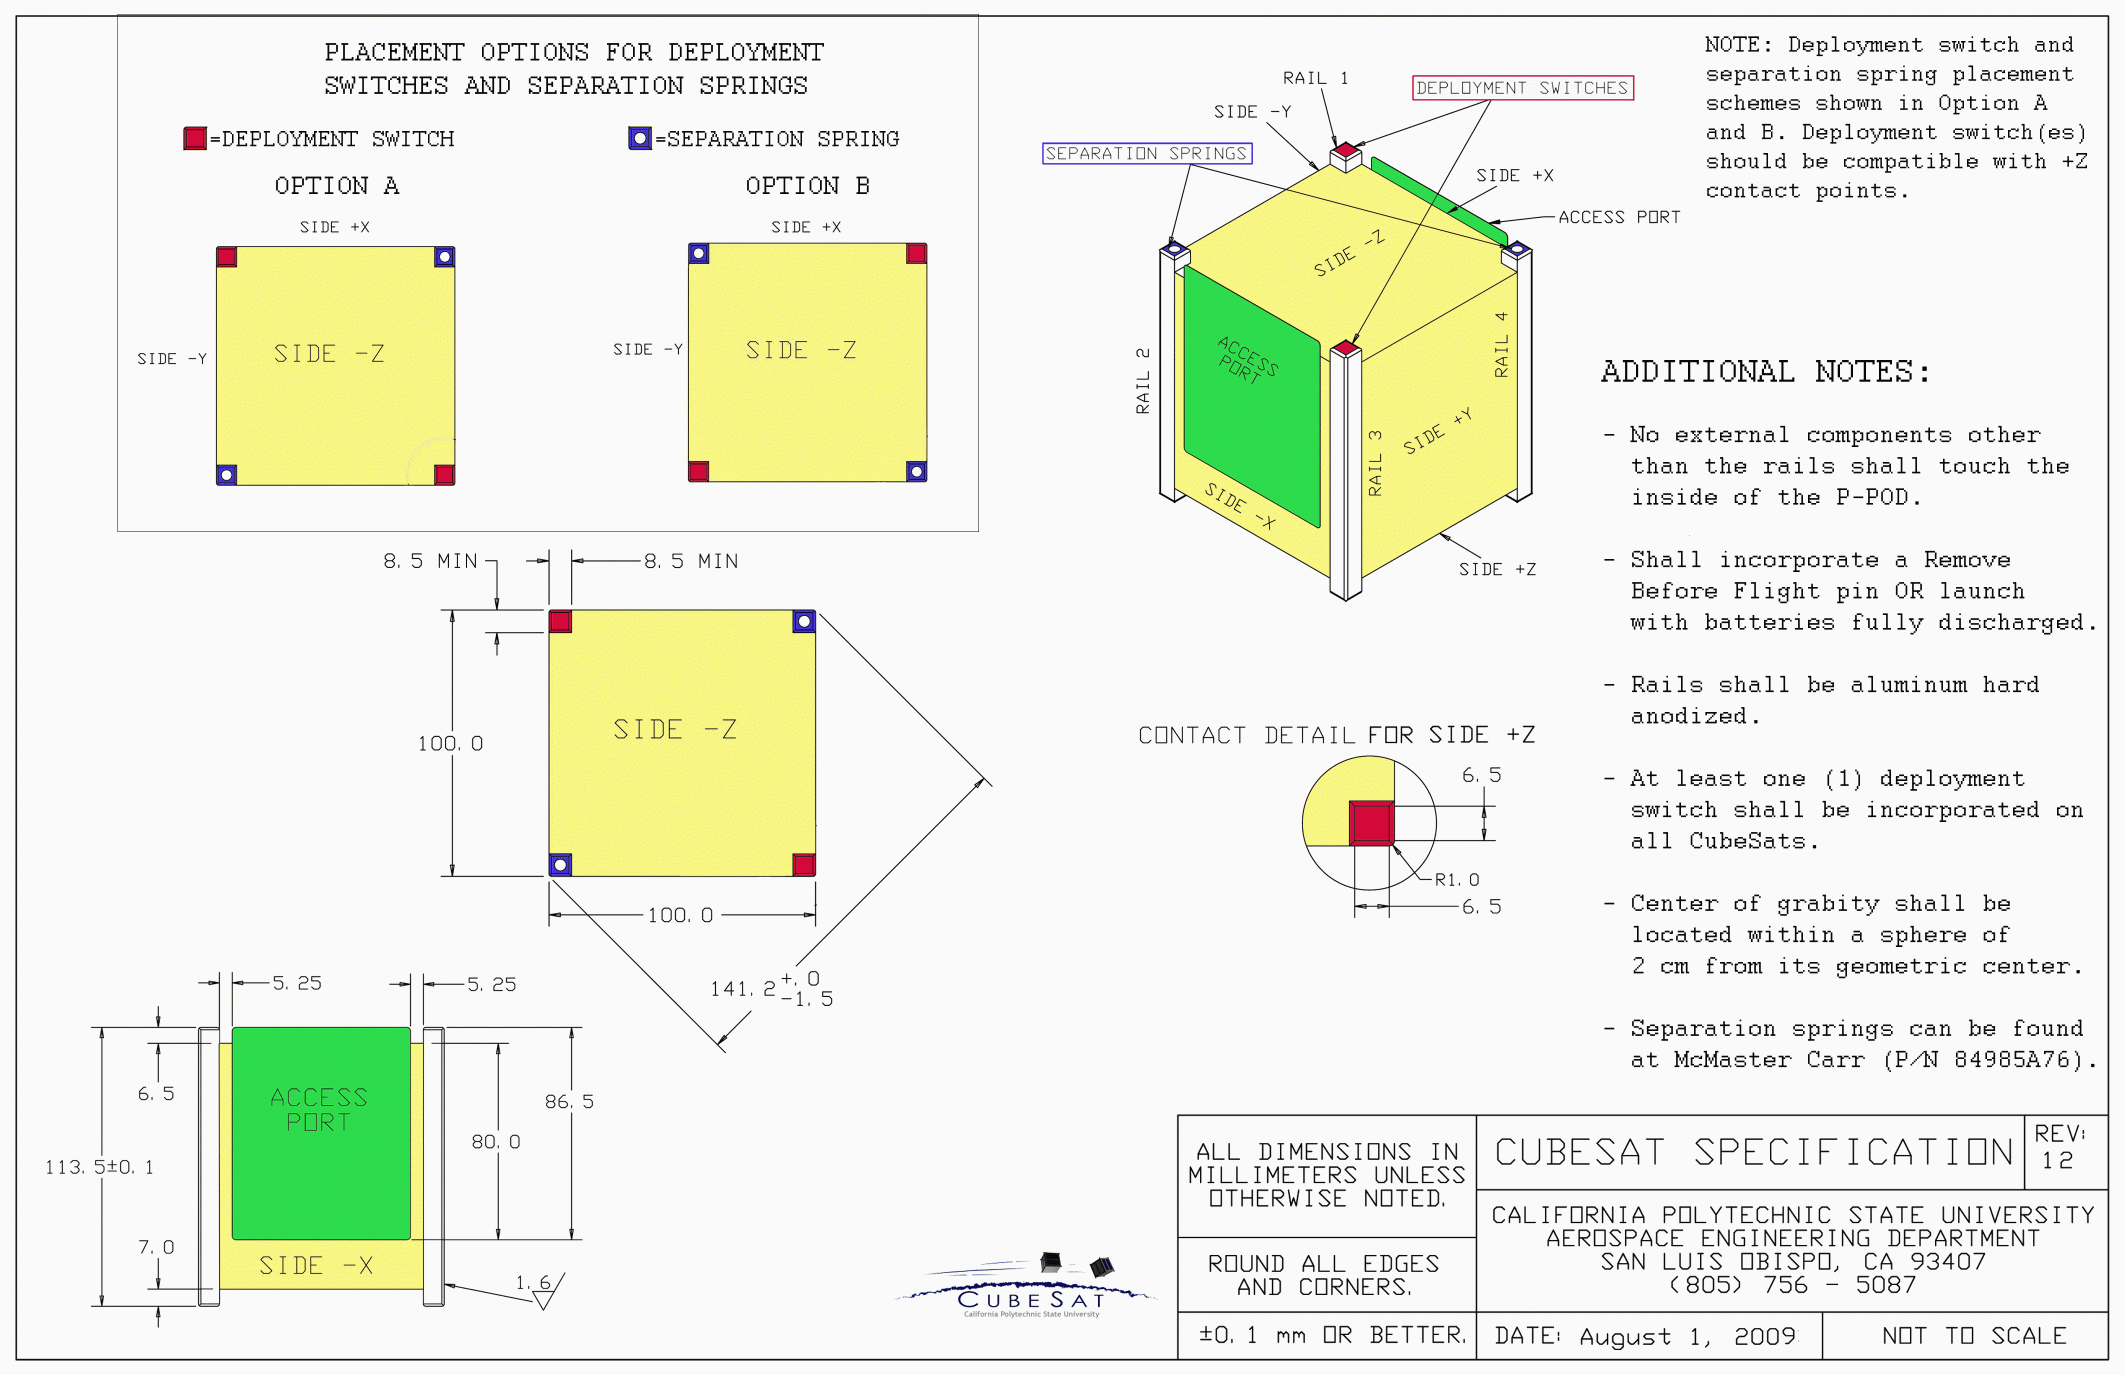
\includegraphics[scale=0.6]{./ANNEXES/images/CubeSatDesign}
\centering
\caption{Dimensions of a 1U CubeSat. Source \cite{cubesatdimensions}}
\label{epsschematics}
\end{figure}

\paragraph{}The two most interesting options that were considered when the structure had to be chosen are presented below.

\begin{longtable}{| l | c | c | }
\hline
\rowcolor[gray]{0.80}	\textbf{Brand and model} &  \textbf{Features}     & \textbf{Total price (\euro)}   \\
\hline
\endfirsthead

\rowcolor[gray]{0.85} \textbf{Structure} &  &  \\
	   ~ISIS 3U structure & \makecell{Low mass (304.3g) \\ Highly compatible \\ High temperature range} & 3900 \\
	   \hline
	   ~Gomspace GOMX-Platform & \makecell{High mass (1500g) \\ Comes fully equipped (basic systems) \\ High temperature range} & 11000 \\
	   \hline
\caption{Options studied for the structure}
\label{structureoptions}
\end{longtable}

\subsection{Thermal protection}
\paragraph{}The thermal protection system consists of various insulating materials that aim to protect the CubeSat from potential thermal shocks. Currently, the most used element as thermal protection in the aerospace industry is the multilayer insulation (MLI), a set of multiple thin insulation layers. The MLI fulfills all the requirements of this mission and its main objective is to reduce the heat generated by radiation, given that the heat generated by convection or conduction does not have such a high impact on the on-board systems.

\paragraph{}A few options were studied when the thermal protection had to be selected. These options are presented in \ref{thermaloptions}
red in this section, the table \ref{structureoptions} is presented below.

\begin{longtable}{| l | c | c | }
\hline
\rowcolor[gray]{0.80}	\textbf{Brand and model} &  \textbf{Features}     & \textbf{Total price (\euro)}   \\
\hline
\endfirsthead
\rowcolor[gray]{0.85} \textbf{Thermal protection} &  &  \\
	   ~Dunmore Aerospace Satkit & \makecell{Lightweight \\ Durability \\ Made for small satellites}& 1000 \\
	   \hline
	   ~Dupont Kapton Aircraft Thermal & \makecell{Lightweight \\ Durability \\ Non-flammable} & 1200 \\
	\hline

\caption{Options studied for the thermal protection}
\label{thermaloptions}
\end{longtable}
